\documentclass[11pt,reqno]{amsart}
\usepackage[T1]{fontenc}
\usepackage{lmodern,amsmath,amssymb,amsthm,mathtools,microtype}
\usepackage[margin=1in]{geometry}
\usepackage{tikz}
\usetikzlibrary{arrows.meta,positioning}
\usepackage{xurl}
\usepackage[hidelinks]{hyperref}
\hypersetup{pdftitle={Influence Bounds for Arbitrary Product Measures},pdfauthor={Deep Bhattacharjee}}
\newtheorem{theorem}{Theorem}[section]
\newtheorem{lemma}[theorem]{Lemma}
\newtheorem{proposition}[theorem]{Proposition}
\newtheorem{corollary}[theorem]{Corollary}
\theoremstyle{definition}
\newtheorem{definition}[theorem]{Definition}
\theoremstyle{remark}
\newtheorem{remark}[theorem]{Remark}
\newcommand{\E}{\mathbb E}
\newcommand{\R}{\mathbb R}
\newcommand{\Var}{\operatorname{Var}}
\newcommand{\one}{\mathbf 1}
\newcommand{\supp}{\operatorname{supp}}
\newcommand{\ag}{\operatorname{ag}}
\newcommand{\cI}{\mathcal I}
\newcommand{\cL}{\mathcal L}
\newcommand{\eps}{\varepsilon}
\newcommand{\abs}[1]{\lvert #1\rvert}
\newcommand{\norm}[1]{\lVert #1\rVert_1}
\DeclareMathOperator{\degint}{deg_{int}}
\numberwithin{equation}{section}
\title[Influence bounds for product measures]{Influence Bounds for Arbitrary Product Measures}
\author{Deep Bhattacharjee}
\address{Formerly, Electro-Gravitational Space Propulsion Laboratory (EGSPL), Bhubaneswar, Odisha 751030, India}
\address{Formerly, University of Calcutta (Heramba Chandra College), 23/49 Gariahat Road, Golpark, Kolkata 700029, West Bengal, India}
\email{d.bhattacharjee@erl-forschung.de}
\email{itsdeep@live.com}
\urladdr{https://orcid.org/0000-0003-0466-750X}
\thanks{Corresponding author: Deep Bhattacharjee, d.bhattacharjee@erl-forschung.de.}
\subjclass[2020]{Primary 68Q12, 60E15; Secondary 06E30, 68Q17}
\keywords{Coordinate influence, product measures, low-degree functions, quantum query complexity}
\begin{document}
\begin{abstract}
Every bounded function of low interaction degree on a finite product space with an arbitrary product measure has a coordinate whose influence is at least a fixed power of its variance, with constants independent of all atom probabilities. As a consequence, low-degree functions under any product measure are approximated by shallow deterministic decision trees. All proofs are complete and self-contained.
\end{abstract}
\maketitle

\section{Introduction}

Aaronson and Ambainis showed that a lower bound on the largest coordinate influence of a bounded low-degree polynomial in terms of its variance would allow quantum algorithms with few queries to be simulated classically on most inputs \cite{AA}. Most results of this kind are proved for the uniform measure on the Boolean cube, or for product measures whose biases stay away from $0$ and $1$, and their constants degrade as the smallest atom probability tends to zero. This paper proves such an influence bound for an arbitrary product measure on an arbitrary finite product, with constants that do not depend on the measure at all.


Let $\Omega=\prod_{i=1}^n\Omega_i$ be a finite product and let
$\mu=\bigotimes_i\mu_i$ be any product probability measure on $\Omega$.
Coordinates with zero atom probabilities and coordinates supported on a single
point are permitted. The function $f$ is defined on the whole product.
For independent $X,Y\sim\mu$, write
$X^{[i]}=(X_1,\ldots,X_{i-1},Y_i,X_{i+1},\ldots,X_n)$ and set
\begin{equation}\label{eq:influences}
 \cI_i(f)=\E\abs{f(X)-f(X^{[i]})}^2,
 \qquad \cL_i(f)=\E\abs{f(X)-f(X^{[i]})}.
\end{equation}
These are independent-resampling quantities. In particular, for fair Boolean
inputs, $\cI_i$ is one half of the squared bit-flip increment.

\begin{definition}
The interaction degree of $f$ is at most $d$ if there is an expansion
\[
 f(x)=\sum_{S\subseteq[n],\ |S|\le d}g_S(x_S)
\]
with real functions $g_S$ depending on the coordinates in $S$.
For Boolean alphabets this is the usual degree of the unique multilinear
polynomial representing $f$.
\end{definition}

Put
\begin{equation}\label{eq:constant}
 c_* =\frac{16\sqrt{15}}{125\pi^4},\qquad
 b=\max\left(1,\left\lceil\log_2\max_i|\Omega_i|\right\rceil\right).
\end{equation}

\begin{theorem}\label{thm:main}
Let $f\colon\Omega\to[0,1]$ have interaction degree at most $d\ge1$.
If $v=\Var_\mu f>0$, then some coordinate satisfies
\begin{equation}\label{eq:main}
 \cI_i(f)\ge c_*\frac{v^{5/2}}{d^6b^4}.
\end{equation}
The constant is independent of $n$, of the measures $\mu_i$, and of their
smallest positive atom probabilities.
\end{theorem}

\begin{corollary}\label{cor:query}
Under the hypotheses of Theorem~\ref{thm:main}, for every
$0<\eps<1/2$ there exists a deterministic decision tree of depth at most
\[
 \min\left(n,\left\lceil\frac{256}{c_*}d^7b^4\eps^{-3}\right\rceil\right)
\]
whose real output $A(X)$ satisfies $\E_\mu(A(X)-f(X))^2\le\eps^2$.
Each query reveals one complete coordinate in $\Omega_i$.
\end{corollary}

Two structural results organize the argument. We state them here and
give complete proofs in Appendices~\ref{app:analytic} and
\ref{app:determinant}, including the analytic estimate needed for the
certificate bound.
For a Boolean cube $Q_k=\{0,1\}^k$ and a function $h$, a row at $u$ is a
nonnegative vector $a^u$ such that
\[
 |h(u)-h(z)|\le\sum_{j:u_j\ne z_j}a_j^u\quad(z\in Q_k).
\]
For Boolean $h$, this says that every block changing its value has weight
at least one.

\begin{proposition}[Turturean's antipodal inequality]\label{prop:external}
Let $h\colon Q_k\to\{0,1\}$ have rows $a^u$. Let $\bar u$ denote the bitwise
complement and let $B_j(h)$ count the unoriented edges in direction $j$
whose endpoints have different values. For all $w_j>0$,
\begin{equation}\label{eq:antipodal}
 \sum_{u:h(u)=1,\ h(\bar u)=0}
 \frac{1}{\sum_j w_j a_j^u a_j^{\bar u}}
 \le\sum_j\frac{B_j(h)}{w_j}.
\end{equation}
Every denominator on the left is positive.
\end{proposition}

Proposition~\ref{prop:external} and its determinant method are due to
Turturean \cite{Turturean}. Appendix~\ref{app:determinant} gives a complete
proof from a determinant of agreement monomials, so the present argument
does not depend on any unpublished source.\footnote{The proof is given in
full so that every step used here can be checked within this paper.}

\begin{proposition}[Agarwal--Ben-David's row bound]\label{prop:rows}
If $F\colon Q_N\to[0,1]$ has polynomial degree at most $D$, it has a row
at every input, each of cost at most $\pi^2D^2/4$.
\end{proposition}

This is the row estimate of Agarwal and Ben-David \cite{ABD}.
Appendix~\ref{app:analytic} proves it using trigonometric interpolation,
Chebyshev polynomials and a finite-dimensional separation argument.
The product transfer, alphabet reduction and query estimate are proved
in the main text. No step assumes an unproved conjecture.

Aaronson and Ambainis established the connection between polynomial
influences and quantum query simulation \cite{AA}. Girish, Mittal, Nehoran
and Raz formulate distributional variants and prove equivalences for fixed
biases \cite{GMNR}. Their Remark 3.5 also treats coordinate-dependent biases
in a fixed interval $[a,1-a]$. Our statement includes arbitrary choices of
the probabilities at each input length, with no such parameter in the bound.

\section{Conditioning two inputs on unordered pairs}

For $x,y\in\Omega$ put $\Delta(x,y)=\{i:x_i\ne y_i\}$.
A row for $f$ at $x\in\Omega$ will mean a vector $a^x\ge0$ with
\begin{equation}\label{eq:product-row}
 |f(x)-f(y)|\le\sum_{i\in\Delta(x,y)}a_i^x\quad(y\in\Omega).
\end{equation}

\begin{lemma}[Product antipodal transfer]\label{lem:pair}
Let $g\colon\Omega\to\{0,1\}$ have rows $a^x$. For any positive weights
$w=(w_i)$,
\begin{equation}\label{eq:product-boolean}
 \E_{X,Y}\frac{\one_{\{g(X)=1,g(Y)=0\}}}
 {\sum_{i\in\Delta(X,Y)}w_i a_i^X a_i^Y}
 \le \frac12\sum_i\frac{\cL_i(g)}{w_i}.
\end{equation}
The integrand is defined to be zero when its numerator is zero.
\end{lemma}

\begin{proof}
Condition on the unordered pair $C_i=\{X_i,Y_i\}$ at every coordinate,
retaining multiplicity when its entries agree. The $C_i$ are independent.
For $C_i=\{s,t\}$ with $s\ne t$, the two orientations have equal conditional
probabilities because
$\mu_i(s)\mu_i(t)=\mu_i(t)\mu_i(s)$.
Consequently, after conditioning, the unequal coordinates form a fair
Boolean cube. Its uniformly chosen vertex represents $X$ and its antipode
represents $Y$. The other coordinates are fixed.

Restrict the rows to the unequal coordinates. They remain valid because
every pair in this cube is also a pair in $\Omega$. Apply
\eqref{eq:antipodal} and divide by the cube size. The normalized number of
boundary edges in a direction is one half of the probability that flipping
that direction changes $g$.

Now average over the $C_i$. The left side becomes the left side of
\eqref{eq:product-boolean}. Flipping one conditional orientation replaces
$X_i$ by $Y_i$, leaving $X_{-i}$ fixed. Before conditioning, $Y_i$ is an
independent sample from $\mu_i$, so the averaged boundary probability is
$\cL_i(g)$. If the conditional cube is a singleton both sides of its
inequality vanish. This proves the claim, including degenerate measures.
\end{proof}

\begin{figure}[tb]
\centering
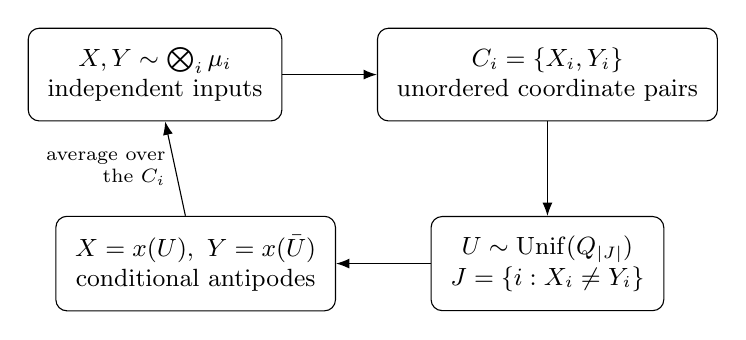
\begin{tikzpicture}[>=Latex,box/.style={draw,rounded corners,align=center,inner sep=7pt,font=\small}]
\node[box] (xy) {$X,Y\sim\bigotimes_i\mu_i$\\independent inputs};
\node[box,right=12mm of xy] (c) {$C_i=\{X_i,Y_i\}$\\unordered coordinate pairs};
\node[box,below=12mm of c] (u) {$U\sim\mathrm{Unif}(Q_{|J|})$\\$J=\{i:X_i\ne Y_i\}$};
\node[box,left=12mm of u] (anti) {$X=x(U),\ Y=x(\bar U)$\\conditional antipodes};
\draw[->] (xy)--(c);
\draw[->] (c)--(u);
\draw[->] (u)--(anti);
\draw[->] (anti)--node[left,font=\scriptsize,align=right]{average over\\the $C_i$}(xy);
\end{tikzpicture}
\caption{The orientations are fair even when the original atom
probabilities are arbitrarily small. Averaging the weighted inequality
precedes the choice of an influential coordinate.}
\end{figure}

\begin{lemma}[Real-valued pair inequality]\label{lem:real}
Let $f\colon\Omega\to\R$ have rows $a^x$, and put
$s_{xy}(w)=\sum_{i\in\Delta(x,y)}w_i a_i^x a_i^y$.
Whenever $f(x)>f(y)$ this denominator is positive. Moreover,
\begin{equation}\label{eq:real}
 \E_{X,Y}\left[\one_{\{f(X)>f(Y)\}}
 \frac{(f(X)-f(Y))^3}{6s_{XY}(w)}\right]
 \le\frac12\sum_i\frac{\cL_i(f)}{w_i}.
\end{equation}
\end{lemma}

\begin{proof}
For a real number $t$ not equal to a value of $f$, let
$g_t(x)=\one_{\{f(x)>t\}}$ and divide the row $a^x$ by $|f(x)-t|$.
If $g_t(x)\ne g_t(y)$, then $|f(x)-f(y)|\ge|f(x)-t|$, so the divided
vector is a row for $g_t$.
Apply Lemma~\ref{lem:pair}. For $f(x)>f(y)$ its summand is
\[
 \one_{\{f(y)<t<f(x)\}}
 \frac{(f(x)-t)(t-f(y))}{s_{xy}(w)}.
\]
The integral of its numerator over $t$ equals $(f(x)-f(y))^3/6$.
Also $\int\cL_i(g_t)\,dt=\cL_i(f)$. Integrating the finite sums gives
\eqref{eq:real}.

For positivity, the divided rows of a Boolean function at differently
valued inputs have positive overlap on some changed coordinate. Indeed,
partition the changed coordinates according to which of the two row
weights is smaller. The intermediate input using one part forces one
of the two sums of smaller weights to be at least one. This also proves
positivity of $s_{xy}(w)$.
\end{proof}

\section{Removing the weights and selecting one coordinate}

\begin{lemma}[A finite-measure calculation]\label{lem:weights}
Let $A,B$ carry positive finite weights $\alpha_x,\beta_y$, and let
$\lambda^x,\nu^y$ be nonnegative vectors. Suppose the quantities
$s_{xy}=\sum_{i\in J(x,y)}w_i\lambda_i^x\nu_i^y$ are positive, and for
every $w_i>0$,
\[
 \sum_{x,y}\frac{\alpha_x\beta_y}{s_{xy}}
 \le C\sum_i\frac1{w_i}.
\]
Then
\begin{equation}\label{eq:remove}
 \left(\sum_x\frac{\alpha_x}{\norm{\lambda^x}}\right)
 \left(\sum_y\frac{\beta_y}{\norm{\nu^y}}\right)\le C.
\end{equation}
\end{lemma}

\begin{proof}
The row norms are positive by the assumption on $s_{xy}$.
Write $v_x=1/\norm{\lambda^x}$, $u_y=1/\norm{\nu^y}$,
$A_0=\sum_x\alpha_xv_x$, $B_0=\sum_y\beta_yu_y$, and
\[
 P_i=\sum_x\alpha_xv_x^2\lambda_i^x,\qquad
 Q_i=\sum_y\beta_yu_y^2\nu_i^y.
\]
Cauchy--Schwarz over the pairs gives
\[
 (A_0B_0)^2\le C\left(\sum_iw_iP_iQ_i\right)
                         \left(\sum_iw_i^{-1}\right).
\]
Here we enlarged $J(x,y)$ to all coordinates in the first factor, whose
terms are nonnegative. Choose $w_i=(\sqrt{P_iQ_i}+\eta)^{-1}$ and let
$\eta\downarrow0$. The right side tends to
$C(\sum_i\sqrt{P_iQ_i})^2\le C(\sum_iP_i)(\sum_iQ_i)=CA_0B_0$.
Division by $A_0B_0>0$ proves the lemma.
\end{proof}

\begin{proposition}[A product certificate bound]\label{prop:certificate}
Suppose $f\colon\Omega\to\R$ has variance $v>0$ and rows of cost at most
$K$ at every point. Put $L=\sum_i\cL_i(f)$. Then $0<L\le K$, and
\begin{equation}\label{eq:certificate}
 \max_i\cI_i(f)\ge\frac{\sqrt{15}}{125}\,
                         \frac{v^{5/2}}{LK^2}.
\end{equation}
\end{proposition}

\begin{proof}
For $M=\max_i\cL_i(f)$ and any $r\in\R$, restrict \eqref{eq:real} to
$A=\{f>r\}$ and $B=\{f\le r\}$. Replacing $(f(x)-f(y))^3$ by
$(f(x)-r)^3$ and multiplying by six gives
\[
 \sum_{x\in A,y\in B}\mu(x)\mu(y)
 \frac{(f(x)-r)^3}{s_{xy}(w)}\le3M\sum_iw_i^{-1}.
\]
Use Lemma~\ref{lem:weights} with
$\lambda^x=a^x/(f(x)-r)^3$ and $\nu^y=a^y$. The norms are at most
$K/(f(x)-r)^3$ and $K$. Hence
\begin{equation}\label{eq:third}
 \E(f-r)_+^3\Pr(f\le r)\le3K^2M.
\end{equation}
Empty sets cause no difficulty. Applying the same statement to $-f$
and choosing a median $m$ gives
$\E|f-m|^3\le12K^2M$. Since
$v\le\E(f-m)^2\le(\E|f-m|^3)^{2/3}$, we obtain
\begin{equation}\label{eq:meanbound}
 \max_i\cL_i(f)\ge\frac{v^{3/2}}{12K^2}.
\end{equation}

For each fixed $x$, averaging the single-coordinate row constraints over
independent replacements shows
$\sum_i\E_{Y_i}|f(x)-f(x_{-i},Y_i)|\le\sum_i a_i^x\le K$.
Thus $L\le K$. If $L=0$, successive averaging over all coordinates makes
$f$ constant almost surely, contrary to $v>0$.

Let
\[
 R=\{i:5L\cI_i(f)<4v\cL_i(f)\},\qquad h=\E[f\mid X_{[n]\setminus R}].
\]
Then $\sum_{i\in R}\cI_i(f)\le4v/5$.
Averaging one coordinate loses variance $\cI_i/2$, and Jensen's inequality
shows that it increases neither resampling quantity of any remaining
coordinate. It follows that $\Var h\ge3v/5$.

Averaging also preserves the row bound. To see this, average the row at
$(x_{-R},z_R)$ over $z_R$, retain its entries outside $R$, and set its
entries in $R$ to zero. Using the same $z_R$ in a comparison of two
inputs proves \eqref{eq:product-row}, with cost at most $K$.
Apply \eqref{eq:meanbound} to $h$. It produces a coordinate $j\notin R$
such that
\[
 \cL_j(f)\ge\cL_j(h)\ge\frac{(3v/5)^{3/2}}{12K^2}.
\]
The definition of $R$ therefore gives
\[
 \cI_j(f)\ge\frac{4v}{5L}\cL_j(f)
 \ge\frac{4}{60}\left(\frac35\right)^{3/2}\frac{v^{5/2}}{LK^2}
 =\frac{\sqrt{15}}{125}\frac{v^{5/2}}{LK^2}.
\]
\end{proof}

The median and averaging steps follow Turturean's strategy. The product
pair transfer is what makes their constants independent of the measures.

\section{Degree estimates and the alphabet reduction}

\begin{lemma}\label{lem:markov}
If $G\colon Q_k\to[0,1]$ has degree at most $d$, then at every vertex $z$,
\begin{equation}\label{eq:local-L1}
 \sum_i|G(z)-G(z^{\oplus i})|\le d^2.
\end{equation}
\end{lemma}

\begin{proof}
Extend $P(s)=2G((s+\one)/2)-1$ multilinearly to $[-1,1]^k$.
It takes values in $[-1,1]$ there. At a vertex $s=2z-\one$,
\[
 \sum_i|G(z)-G(z^{\oplus i})|=\sum_i|\partial_iP(s)|.
\]
Choose $y_i$ to be the sign of $\partial_iP(s)$.
Lemma~\ref{lem:banach-markov} bounds $|DP(s)[y]|$ by $d^2$,
which is the desired sum. This is the pointwise inequality of
Filmus, Hatami, Keller and Lifshitz \cite{FHKL}, with the normalization
used here.
\end{proof}

\begin{lemma}\label{lem:L}
For every $f\colon\Omega\to[0,1]$ of interaction degree at most $d$,
\[
 \sum_i\cL_i(f)\le d^2.
\]
\end{lemma}

\begin{proof}
For fixed endpoints $x,y$, restrict $f$ to the cube which chooses either
$x_i$ or $y_i$ at each coordinate. Its Boolean polynomial degree is at
most $d$, because every component $g_S$ depends on at most $d$ of the
choice bits. Apply Lemma~\ref{lem:markov} at the vertex corresponding to
$x$. Averaging over independent $x,y\sim\mu$ gives the claim exactly.
\end{proof}

\begin{lemma}\label{lem:encoding}
If $f\colon\Omega\to[0,1]$ has interaction degree at most $d$, then it
has rows on $\Omega$ of cost at most $\pi^2d^2b^2/4$.
\end{lemma}

\begin{proof}
Choose a surjection $D_i\colon\{0,1\}^b\to\Omega_i$ at each coordinate,
and let $D=(D_1,\ldots,D_n)$. The Boolean function $F=f\circ D$ takes
values in $[0,1]$ everywhere. Each component $g_S\circ D$ depends on
at most $b|S|$ Boolean bits, so its degree is at most $bd$. Thus
Proposition~\ref{prop:rows} supplies rows $\alpha^u$ for $F$ of cost
at most $\pi^2d^2b^2/4$.

Fix a section $e_i\colon\Omega_i\to\{0,1\}^b$ of $D_i$.
At $x\in\Omega$ define
$a_i^x=\sum_{j=1}^b\alpha_{ij}^{e(x)}$.
For any $y$, the codes $e(x),e(y)$ agree outside the blocks
$i\in\Delta(x,y)$. The Boolean row inequality bounds
$|F(e(x))-F(e(y))|=|f(x)-f(y)|$ by the sum of these block weights.
The total cost equals the cost of $\alpha^{e(x)}$, proving the lemma.
The codes are used only for this certificate argument. They impose no
condition on $\mu$.
\end{proof}

\begin{proof}[Proof of Theorem~\ref{thm:main}]
Insert $L\le d^2$ and $K\le\pi^2d^2b^2/4$ into
\eqref{eq:certificate}. Their product satisfies
$LK^2\le\pi^4d^6b^4/16$, giving \eqref{eq:main}.
\end{proof}

\section{Decision trees and quantum queries}

We record the product orthogonal decomposition explicitly. For every
coordinate, take an orthonormal basis of $L^2(\mu_i)$ whose first element
is the constant one. Products of these basis elements form an
orthonormal basis of $L^2(\mu)$. Grouping by the set of coordinates with
nonconstant basis elements gives
\[
 f=\sum_{S\subseteq[n]}f_S,\qquad
 \E[f_S\mid X_{[n]\setminus\{i\}}]=0\quad(i\in S).
\]
All summands with $|S|>d$ vanish for a function of interaction degree $d$.
Parseval and independent resampling yield
\begin{equation}\label{eq:anova}
 \Var f=\sum_{S\ne\varnothing}\|f_S\|_2^2,\qquad
 \cI_i(f)=2\sum_{S\ni i}\|f_S\|_2^2,
 \qquad\sum_i\cI_i(f)\le2d\Var f.
\end{equation}
Zero-mass atoms are omitted when forming these $L^2$ bases.

\begin{proof}[Proof of Corollary~\ref{cor:query}]
At every nonconstant node query a remaining coordinate of largest
resampling influence for the conditional function and product law.
Constant nodes become leaves. Queries preserve the degree bound.
Let $\rho_t$ be the resulting random restriction after depth $t$, and
write
\[
 D_t=\E\Var(f\mid\rho_t),\qquad
 P_t=\E\sum_{j\text{ unqueried}}\cI_j(f\mid\rho_t).
\]
Once a branch ends we pad it with no operation. By
\eqref{eq:anova}, $P_t\le2dD_t$, and $D_t$ is nonincreasing.
If the next query at a node is $i$, then for every $j\ne i$ the average
conditional value of $\cI_j$ equals its value before that query.
This follows by writing its two-copy expectation and first averaging
over $X_i$. Thus
\begin{equation}\label{eq:potential}
 P_t-P_{t+1}=\E\cI_{i(\rho_t)}(f\mid\rho_t).
\end{equation}

Suppose a stage begins with $D_t\le u$ and continues while $D_t>u/2$.
Let $V=\Var(f\mid\rho_t)$ and $V_+=V\one_{\{V\ge u/4\}}$.
The contribution from $V<u/4$ is at most $u/4$, so
$\E V_+>u/4$. Theorem~\ref{thm:main} and Jensen's inequality imply
\[
 P_t-P_{t+1}\ge\frac{c_*}{d^6b^4}\E V^{5/2}
 \ge\frac{c_*u^{5/2}}{32d^6b^4}.
\]
The potential at the beginning of the stage is at most $2du$.
Therefore at most
$\lfloor64d^7b^4/(c_*u^{3/2})\rfloor+1$ levels are needed to make
$D_t\le u/2$.

Start with $u_0=1/4$ and halve $u$ until $u\le\eps^2$.
If $J$ stages are needed, then $u_{J-1}>\eps^2$ and
\[
 \sum_{j=0}^{J-1}u_j^{-3/2}
 <\frac{\eps^{-3}}{1-2^{-3/2}}<2\eps^{-3}.
\]
Since $64d^7b^4/(c_*u^{3/2})>1$, each extra rounding term can
be absorbed by doubling this stage bound. The stated depth follows.
At a leaf output $\E[f\mid\rho]$. Its total mean-square error is
$\E\Var(f\mid\rho)\le\eps^2$. If the depth bound exceeds $n$, querying
all inputs gives exact evaluation instead.
\end{proof}

\begin{corollary}\label{cor:quantum}
Let a quantum query algorithm make $T\ge1$ queries to a finite-alphabet
input, with each query returning one symbol, and let $p(x)$ be its
acceptance probability on every input. Under every product input law,
there exists a deterministic classical tree of depth
$O(T^7b^4\eps^{-3})$ with mean-square error at most $\eps^2$ in estimating
$p$. For $0<\eta,\delta<1$, a depth
$O(T^7b^4\eta^{-3}\delta^{-3/2})$ suffices for error at most $\eta$
outside a set of probability at most $\delta$.
\end{corollary}

\begin{proof}
The polynomial method \cite{BBCMW} gives interaction degree at most
$2T$. For completeness, each oracle matrix entry is a function of one
input symbol. After $T$ queries every amplitude is a sum of terms each
depending on at most $T$ input coordinates. Squaring amplitudes and
summing over accepting states gives interaction degree at most $2T$.
Intermediate measurements can be deferred using an auxiliary register.
Corollary~\ref{cor:query} with $d=2T$ proves the first statement.
For the second use $\eps=\eta\sqrt\delta$ and apply Markov's inequality
to the squared estimation error. Values of $\eps\ge1/2$ can be replaced
by a constant-output estimate.
\end{proof}

The tree can use exact conditional expectations and an exhaustive
description of the input function. The conclusion controls the number
of input queries. It gives no bound on the computation required to
construct the tree or its numerical leaf values.

\section{The sharp variance question}

\begin{proposition}[The optimal linear case]\label{prop:linear}
Let $f\colon\Omega\to[0,1]$ have interaction degree at most one and
variance $v>0$. Then
\[
 \max_i\cI_i(f)\ge8v^2.
\]
The constant eight is optimal, even for fair Boolean inputs.
\end{proposition}

\begin{proof}
Write $f=c+\sum_i g_i(x_i)$ and put
$r_i=\max g_i-\min g_i$. Independence gives
$v=\sum_i v_i$, where $v_i=\Var(g_i(X_i))$, and
$\cI_i(f)=2v_i$.
Because all combinations of coordinate values belong to the domain,
$\sum_i r_i=\max f-\min f\le1$.
The variance bound for a variable in an interval of length $r_i$ gives
$\sqrt{v_i}\le r_i/2$. If $M=\max_i\cI_i(f)$, then
\[
 v=\sum_i v_i\le\sqrt{M/2}\sum_i\sqrt{v_i}
 \le\frac12\sqrt{M/2}.
\]
Squaring yields the claim. For $f(x)=n^{-1}\sum_i x_i$ on the fair
Boolean cube, $v=1/(4n)$ and $\cI_i=1/(2n^2)=8v^2$.
\end{proof}

This example also precludes any influence bound with variance exponent
smaller than two and a degree-dependent positive constant. A bound with
exponent two and polynomial dependence on arbitrary degree remains an
open question; the arguments here give the exponent $5/2$.

\appendix
\section{Analytic estimates and certificate rows}\label{app:analytic}

We give the analytic chain from finite interpolation to
Proposition~\ref{prop:rows}. This also proves the precise pointwise
estimate used in Lemma~\ref{lem:markov}.

\subsection{Trigonometric interpolation}

\begin{lemma}[Bernstein's inequality for trigonometric polynomials]\label{lem:trig}
If $H(\theta)=\sum_{j=-D}^D h_j e^{ij\theta}$, with $D\ge1$, then
\[
 |H'(\theta)|\le D\sup_{t\in\R}|H(t)|.
\]
\end{lemma}

\begin{proof}
It is enough to evaluate the derivative at zero, since translating
$H$ leaves its degree and supremum unchanged. Put
\[
 t_k=\frac{(2k-1)\pi}{2D},\qquad
 c_k=\frac{(-1)^{k-1}}{4D\sin^2(t_k/2)},\qquad 1\le k\le2D.
\]
We claim that
\begin{equation}\label{eq:riesz}
 H'(0)=\sum_{k=1}^{2D}c_k H(t_k).
\end{equation}
Here is a finite verification. Orthogonality on this shifted grid shows
that the coefficient which differentiates the modes
$e^{ij\theta}$ for $-D+1\le j\le D$ is
\[
 c_k=\frac1{2D}\sum_{j=-D+1}^D ij e^{-ijt_k}.
\]
Indeed, the sum over $k$ of $e^{i(j-r)t_k}$ is zero unless $j=r$
for indices in that interval. The remaining mode $j=-D$ has sampled
values equal to the negative of the sampled values of $j=D$, and its
derivative at zero is also the negative, so it obeys the same formula.

To compute the coefficient, set $z=e^{-it_k}$, so $z^{2D}=-1$.
Differentiating the finite geometric sum gives
\[
 \sum_{j=-D+1}^D jz^j
 =z\frac{d}{dz}\left(z^{-D+1}\frac{1-z^{2D}}{1-z}\right)
 =\frac{2z^{-D+1}}{(1-z)^2}
 \quad\text{at }z^{2D}=-1.
\]
Since $(1-z)^2=-4z\sin^2(t_k/2)$ and
$e^{iDt_k}=i(-1)^{k-1}$, this is precisely the displayed value of $c_k$.
This proves \eqref{eq:riesz} without an interpolation remainder.

Apply the identity to $H(\theta)=\sin(D\theta)$.
Because $\sin(Dt_k)=(-1)^{k-1}$, it gives
$\sum_k|c_k|=D$. Taking absolute values in \eqref{eq:riesz}
now proves the lemma.
\end{proof}

\subsection{A derivative estimate on the solid cube}

\begin{lemma}\label{lem:banach-markov}
Let $P\colon\R^N\to\R$ be a polynomial of total degree at most $d$
and assume $|P|\le1$ on $[-1,1]^N$. If $x,y\in[-1,1]^N$, then
\begin{equation}\label{eq:cube-markov}
 |DP(x)[y]|\le d^2.
\end{equation}
\end{lemma}

\begin{proof}
The case $d=0$ is immediate. For $-1<r<1$ consider
\[
 H_r(\theta)=P\bigl(rx\cos\theta+\sqrt{1-r^2}\,y\sin\theta\bigr).
\]
Its argument lies in the solid cube. For each coordinate this follows
from Cauchy--Schwarz applied to $(r,\sqrt{1-r^2})$ and
$(x_i\cos\theta,y_i\sin\theta)$. It is a trigonometric polynomial
of degree at most $d$, with supremum at most one. Thus
Lemma~\ref{lem:trig} gives
\[
 \sqrt{1-r^2}\,|DP(rx)[y]|=|H_r'(0)|\le d.
\]
The function $g(r)=DP(rx)[y]$ is a polynomial of degree at most $d-1$.
Consequently $G(\theta)=\sin\theta\,g(\cos\theta)$ is a
trigonometric polynomial of degree at most $d$ and satisfies $|G|\le d$.
Apply Lemma~\ref{lem:trig} once more. Since $G'(0)=g(1)$, it gives
$|DP(x)[y]|\le d^2$.
\end{proof}

The intermediate estimate also explains why the boundary of the cube
requires care. The first use of Bernstein loses
$(1-r^2)^{-1/2}$ as $r$ approaches one. Multiplication by
$\sin\theta$ and the second finite interpolation bound remove that loss.
\footnote{The proof uses total polynomial degree before restricting to
vertices. Replacing a Boolean power by its multilinear representative
can only decrease that degree.}

\subsection{Chebyshev polynomials and overlapping blocks}

Define $T_0(t)=1$, $T_1(t)=t$, and
$T_{m+1}(t)=2tT_m(t)-T_{m-1}(t)$.
The cosine addition identity proves inductively that
$T_m(\cos\theta)=\cos(m\theta)$.
In particular $\deg T_m=m$, $|T_m|\le1$ on $[-1,1]$,
$T_m(1)=1$ and $T_m(\cos(\pi/m))=-1$ for $m\ge1$.

For a function $F$ on the sign cube with values in $[0,1]$, its
multilinear extension $\widetilde F$ has the exact formula
\begin{equation}\label{eq:multiaffine}
 \widetilde F(u)=\sum_{z\in\{-1,1\}^N}
          F(z)\prod_i\frac{1+z_i u_i}{2}.
\end{equation}
The coefficients in this sum are nonnegative and add to one on the
solid cube. Thus its extension still takes values in $[0,1]$ there.

\begin{lemma}[Block bound]\label{lem:blocks}
Let $F\colon\{-1,1\}^N\to[0,1]$ have degree at most $D$, and fix a vertex
$x$. Let $S_1,\ldots,S_k$ be a list of coordinate sets in which each
coordinate occurs at most $N_0$ times. If $m\ge1$ and
$N_0(1-\cos(\pi/m))\le2$, then
\begin{equation}\label{eq:block-bound}
 \sum_{a=1}^k |F(x)-F(x^{S_a})|\le D^2m^2.
\end{equation}
\end{lemma}

\begin{proof}
For $w\in\{-1,1\}^k$ put
\[
 \nu_i(w)=\sum_{a:i\in S_a}\frac{1-w_a}{2},\qquad
 \theta_i(w)=T_m\bigl(1-(1-\cos(\pi/m))\nu_i(w)\bigr),
\]
and define
$G(w)=\widetilde F(x_1\theta_1(w),\ldots,x_N\theta_N(w))$.
Because $0\le\nu_i\le N_0$, the arguments of every $T_m$ lie in
$[-1,1]$. Formula~\eqref{eq:multiaffine} implies $0\le G\le1$.
Each $\theta_i$ has polynomial degree at most $m$, so $G$ has degree
at most $Dm$ after multilinearization.

At the all-one vertex, every $\theta_i=1$ and $G(\one)=F(x)$.
Changing just coordinate $a$ of $w$ changes $\theta_i$ to $-1$
exactly for $i\in S_a$. Thus $G(\one^{\oplus a})=F(x^{S_a})$.
The pointwise bound of Lemma~\ref{lem:markov}, which follows from
Lemma~\ref{lem:banach-markov}, gives \eqref{eq:block-bound}.
\end{proof}

\begin{lemma}[Fractional block packing]\label{lem:packing}
Fix $F$ and $x$ as above. If $\lambda_S\ge0$ and
$\sum_{S\ni i}\lambda_S\le1$ for every coordinate $i$, then
\[
 \sum_S\lambda_S|F(x)-F(x^S)|\le\frac{\pi^2}{4}D^2.
\]
\end{lemma}

\begin{proof}
For an integer $M\ge1$, put $N_0=M^2$ and
$m=\lceil\pi M/2\rceil$. Make a list in which each block $S$ occurs
$\lfloor M^2\lambda_S\rfloor$ times. Each coordinate occurs at most
$N_0$ times, and
\[
 N_0(1-\cos(\pi/m))\le\frac{M^2\pi^2}{2m^2}\le2.
\]
Apply Lemma~\ref{lem:blocks} and divide by $M^2$.
For this fixed finite family the left side converges to the asserted
packing sum, while $m^2/M^2\to\pi^2/4$.
\end{proof}

\subsection{Finite separation and the row estimate}

We include the separation step to make explicit why one row can cover
every target input simultaneously.

\begin{lemma}\label{lem:finite-separation}
Let $C\subset\R^m$ be nonempty, compact and convex, with no point in
$[0,\infty)^m$. Then there is a nonzero vector $\kappa\ge0$ such that
$\langle\kappa,c\rangle<0$ for every $c\in C$.
\end{lemma}

\begin{proof}
Minimize $\rho(c)=\sum_s\max(-c_s,0)^2$ on $C$, at a point $y$.
Its minimum is positive. Let $\kappa_s=\max(-y_s,0)$, so
$y+\kappa\ge0$ and $\langle\kappa,y\rangle=-\rho(y)$.
For $c\in C$ and $0<t\le1$, convexity and minimality give
\[
 \rho(y)\le\rho(y+t(c-y))
 \le\|t(c-y)-\kappa\|_2^2.
\]
Subtract $\rho(y)$, divide by $t$ and let $t\downarrow0$.
It follows that $\langle\kappa,c-y\rangle\le0$, proving the claim.
\end{proof}

\begin{proof}[Proof of Proposition~\ref{prop:rows}]
Use the sign-cube coordinates, which do not change degree, and fix $x$.
Set $t_S=|F(x)-F(x^S)|$ and $K=\pi^2D^2/4$.
Let $P=\{a\ge0:\sum_i a_i\le K\}$ and consider the compact convex set
\[
 C=\left\{\left(\sum_{i\in S}a_i-t_S\right)_{S\subseteq[N]}:a\in P\right\}.
\]
If $C$ meets the nonnegative orthant, the corresponding $a$ is the
required row. Otherwise Lemma~\ref{lem:finite-separation} produces
$\kappa_S\ge0$ with
\[
 \sum_i a_i\sigma_i<\tau\quad(a\in P),\qquad
 \sigma_i=\sum_{S\ni i}\kappa_S,\quad \tau=\sum_S\kappa_St_S.
\]
Taking $a=0$ shows $\tau>0$. Since $t_\varnothing=0$, some
$\sigma_i$ is positive. Let $j$ maximize $\sigma_i$.
The weights $\lambda_S=\kappa_S/\sigma_j$ form a fractional packing,
so Lemma~\ref{lem:packing} gives $\tau\le K\sigma_j$.
Taking $a=Ke_j$ gives the strict reverse inequality, a contradiction.
\end{proof}

\section{The determinant proof of the antipodal inequality}\label{app:determinant}

We give Turturean's determinant construction in the notation required
for the product transfer. Throughout this appendix all matrices have
finite index sets and polynomial entries over $\R$.

\subsection{Agreement monomials and lowest terms}

Let $O\subseteq Q_k$ and let $b_j$ count its boundary edges in direction
$j$. Write $\ag(x,z)=\{j:x_j=z_j\}$ and
$s^A=\prod_{j\in A}s_j$. The agreement matrix is
\[
 M[x,z]=s^{\ag(x,z)},\qquad x,z\in O.
\]
A lowest term of a nonzero polynomial means a monomial with nonzero
coefficient of minimum total degree. If a polynomial $u$ has constant
term one, multiplication by $u$ leaves the whole lowest homogeneous
part of any nonzero polynomial unchanged. We will use this observation
when comparing determinants.

\begin{lemma}\label{lem:lowest-det}
The determinant of $M$ is nonzero. Every lowest term $s^\gamma$ of
$\det M$ satisfies $\gamma_j\le b_j$ for all $j$.
\end{lemma}

\begin{proof}
If $O$ is empty, its determinant is one. Otherwise specialize every
$s_j$ to $c=2^k$. The diagonal entry of each row is $c^k$.
Each off-diagonal entry is at most $c^{k-1}$, and there are
$|O|-1<c$ of them. The resulting real matrix is strictly diagonally
dominant, and hence nonsingular. For a direct verification, a nonzero
null vector would have a component of maximum absolute value whose row
equation contradicts strict dominance. Therefore $\det M$ is nonzero.

Fix $j$, and let $e_j$ be the number of pairs $\{x,x^{\oplus j}\}$
entirely contained in $O$. Subtract $s_j$ times the row at
$x^{\oplus j}$ from the row at $x$ whenever $x_j=1$ and both rows
belong to $O$. These operations affect disjoint pairs and leave the
determinant unchanged. In each changed row the entries at columns
with $z_j=x_j$ vanish. The other entries are
$(1-s_j^2)M[x,z]$. Consequently
\[
 \det M=(1-s_j^2)^{e_j}R_j
\]
for a polynomial $R_j\ne0$.
Each matrix entry has degree at most one in $s_j$, so
$\deg_{s_j}\det M\le |O|=2e_j+b_j$.
The leading coefficient of a product of nonzero polynomials in $s_j$
cannot vanish. Thus $\deg_{s_j}R_j\le b_j$.
Since $(1-s_j^2)^{e_j}$ has constant term one, the lowest homogeneous
parts of $\det M$ and $R_j$ coincide. The asserted exponent bound
follows for this $j$ and therefore for every coordinate.
\end{proof}

\subsection{A permutation respecting local subcubes}

Call $A_x\subseteq[k]$ a wing at $x\in O$ when $x^S\in O$ for every
$S\subseteq A_x$.

\begin{lemma}[Turturean's permutation construction]\label{lem:permutation}
For any wing $A_x$ at every $x\in O$, there is a permutation
$\tau\colon O\to O$ such that
\[
 \tau(x)_j\ne x_j\quad(j\in A_x),\qquad
 \#\{x\in O:\tau(x)_j=x_j\}\le b_j\quad(j\in[k]).
\]
\end{lemma}

\begin{proof}
Define matrices indexed by $O$ by
\begin{align*}
 P[x,z]&=\begin{cases}(-1)^{|\Delta(x,z)|}s^{\Delta(x,z)},
                      &\Delta(x,z)\subseteq A_x,\\0,&\text{otherwise},\end{cases}\\
 U[x,x]&=\prod_{i\in A_x}(1-s_i^2),\qquad U[x,z]=0\quad(x\ne z),\\
 Q[x,z]&=\begin{cases}s^{\ag(x,z)},&\ag(x,z)\cap A_x=\varnothing,\\
                       0,&\text{otherwise}.
                       \end{cases}
\end{align*}
Summing the row combinations of $M$ coordinate by coordinate gives
\begin{equation}\label{eq:wing-matrix}
 PM=UQ.
\end{equation}
To check an entry, sum over $S\subseteq A_x$ the quantities
$(-1)^{|S|}s^S s^{\ag(x^S,z)}$. For $i\in A_x$, its two local terms
are $s_i-s_i=0$ when $x_i=z_i$, and $1-s_i^2$ otherwise. The remaining
coordinates retain their agreement monomials. This is exactly the
entry of $UQ$. The wing property ensures every row $x^S$ used in this
sum belongs to $O$.

At $s=0$, $P$ is the identity, and each diagonal entry of $U$ is one.
Their determinants therefore have constant term one. Taking
determinants in \eqref{eq:wing-matrix} shows that $\det Q\ne0$ and that
its lowest homogeneous part equals that of $\det M$.
Choose a lowest monomial of $\det Q$. The determinant expansion has at
least one permutation whose nonzero product of entries contributes to
that monomial. Let this permutation be $\tau$.
Its nonzero entries ensure $\ag(x,\tau(x))\cap A_x=\varnothing$.
The exponent of $s_j$ in its product is exactly the number of inputs
at which $\tau(x)_j=x_j$. Lemma~\ref{lem:lowest-det} bounds it by $b_j$.
\end{proof}

\begin{figure}[tb]
\centering
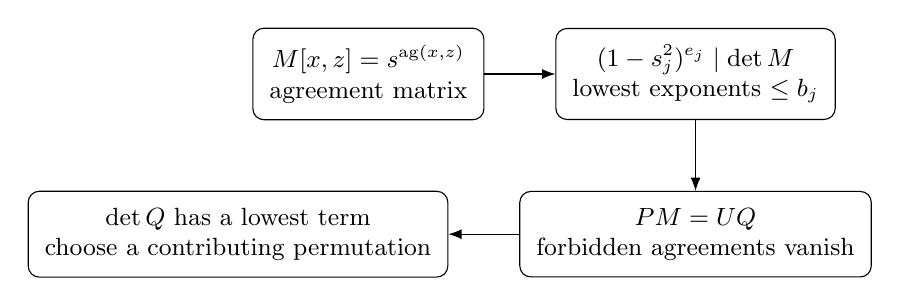
\begin{tikzpicture}[>=Latex,node distance=7mm,
 box/.style={draw,rounded corners,align=center,inner sep=6pt,font=\small}]
\node[box] (m) {$M[x,z]=s^{\ag(x,z)}$\\agreement matrix};
\node[box,right=9mm of m] (factor) {$(1-s_j^2)^{e_j}\mid\det M$\\lowest exponents $\le b_j$};
\node[box,below=9mm of factor] (wing) {$PM=UQ$\\forbidden agreements vanish};
\node[box,left=9mm of wing] (perm) {$\det Q$ has a lowest term\\choose a contributing permutation};
\draw[->] (m)--(factor);
\draw[->] (factor)--(wing);
\draw[->] (wing)--(perm);
\end{tikzpicture}
\caption{The determinant construction supplies one permutation satisfying
all coordinate budgets simultaneously. The construction and its
antipodal consequence are due to Turturean.}
\end{figure}

\subsection{From the permutation to rows}

Let $h=\one_O$ and $Z=\{u\in O:\bar u\notin O\}$.
For positive lengths $\ell_j$ and a wing $A$ at $u\in Z$, put
\[
 D(u,A)=\min\left\{\sum_{j\in G}\ell_j:
              G\subseteq[k]\setminus A,\ \bar u^{G}\in O\right\}.
\]
The minimum exists because $G=[k]\setminus A$ gives
$\bar u^G=u^A\in O$.

\begin{lemma}\label{lem:wing-budget}
For any wings $A_u$ at $u\in Z$,
\[
 \sum_{u\in Z}D(u,A_u)\le\sum_j\ell_j b_j.
\]
\end{lemma}

\begin{proof}
Take empty wings on $O\setminus Z$ and apply
Lemma~\ref{lem:permutation}. For $u\in Z$, the set
$G_u=\ag(u,\tau(u))$ is disjoint from $A_u$ and satisfies
$\bar u^{G_u}=\tau(u)\in O$. Thus
$D(u,A_u)\le\sum_{j\in G_u}\ell_j$.
Sum over $u$, enlarge the sum to $O$, and use the coordinate budgets
of that permutation.
\end{proof}

We also need positivity of the overlap of two Boolean rows.
Let $h(u)=1$, $h(v)=0$, and let $a,b$ be rows at $u,v$.
Put $D=\Delta(u,v)$ and $S=\{j\in D:a_j\le b_j\}$.
The input $u^S=v^{D\setminus S}$ has one of the two Boolean values.
If its value is zero, $a(S)\ge1$. Otherwise $b(D\setminus S)\ge1$.
In both cases
\begin{equation}\label{eq:overlap}
 \sum_{j\in D}\min(a_j,b_j)\ge1.
\end{equation}
In particular there is a coordinate with $a_jb_j>0$.

\begin{proof}[Proof of Proposition~\ref{prop:external}]
For $u\in Z$, write $a=a^u$, $b=a^{\bar u}$ and
$\ell_j=w_j^{-1}$. Equation~\eqref{eq:overlap} ensures
$s_u=\sum_j a_jb_j/\ell_j>0$. Set $\omega_u=s_u^{-1}$ and choose
\[
 A_u=\{j:\ell_j<\omega_u b_j\}.
\]
Because $\sum_j a_j\omega_u b_j/\ell_j=1$, we have
$\sum_{j\in A_u}a_j<1$. If all those $a_j$ vanish the claim is
immediate, and otherwise it follows from the strict inequalities in
the definition of $A_u$. Every subset of $A_u$ therefore leaves the
value at $u$ equal to one, so $A_u$ is a wing.

If $G\subseteq[k]\setminus A_u$ and $\bar u^G\in O$, the row at
$\bar u$ gives $\sum_{j\in G}b_j\ge1$.
For each such coordinate $\ell_j\ge\omega_u b_j$, whence
$\sum_{j\in G}\ell_j\ge\omega_u$. Thus $D(u,A_u)\ge\omega_u$.
Lemma~\ref{lem:wing-budget} now gives
\[
 \sum_{u\in Z}\frac1{\sum_j w_j a_j^u a_j^{\bar u}}
 \le\sum_{u\in Z}D(u,A_u)\le\sum_j\frac{b_j(h)}{w_j},
\]
which is the required inequality.
\end{proof}

\section{Examples and the limits of averaging}

\subsection{A rare-coordinate calculation}
For $f(x)=x_1$ under any Bernoulli product law,
\[
 v=p_1(1-p_1),\qquad\cI_1=2p_1(1-p_1)=2v,
 \qquad\cI_i=0\quad(i>1).
\]
As $p_1\to0$ the variance and the relevant influence vanish together.
Theorem~\ref{thm:main} continues to apply with its fixed constant.
At $p_1=0$ the variance is zero and no positive lower bound is asserted.
\footnote{A bound uniform in the probabilities need not give a fixed
positive influence when its own variance parameter tends to zero. The
quantifiers require the displayed variance-dependent estimate at every
choice of probabilities.}

\subsection{A two-coordinate interaction}
For $f(x)=x_1x_2$ with independent probabilities $p,q$,
\[
 v=pq(1-pq),\qquad
 \cI_1=2p(1-p)q,\qquad\cI_2=2q(1-q)p.
\]
This checks that resampling retains the unchanged coordinate in both
copies of the increment. Using a completely independent second input
instead would give a different quantity.

\subsection{Why the order of the proof matters}
Applying an influence theorem separately in each conditional cube
only gives a lower bound on the average of a maximum. In general this
does not lower bound the maximum of the averages. For example, if
$J$ is uniform on $[n]$ and $a_i(J)=\one_{\{i=J\}}$, then
$\E\max_i a_i(J)=1$ but $\max_i\E a_i(J)=1/n$.
The argument of Lemma~\ref{lem:pair} avoids this loss by keeping every
positive coordinate weight until after averaging. The finite-measure
calculation then chooses the weights for the original product law.

\begin{figure}[tb]
\centering
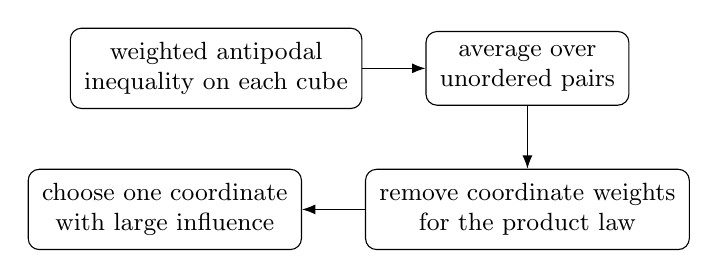
\begin{tikzpicture}[>=Latex,box/.style={draw,rounded corners,align=center,inner sep=5pt,font=\small}]
\node[box] (weighted) {weighted antipodal\\inequality on each cube};
\node[box,right=8mm of weighted] (average) {average over\\unordered pairs};
\node[box,below=8mm of average] (remove) {remove coordinate weights\\for the product law};
\node[box,left=8mm of remove] (select) {choose one coordinate\\with large influence};
\draw[->] (weighted)--(average);
\draw[->] (average)--(remove);
\draw[->] (remove)--(select);
\end{tikzpicture}
\caption{The coordinate is selected after the product average. This order
prevents a dimension-dependent loss from the changing maximizing index.}
\end{figure}

\section{Variance calculations used in the proof}

\subsection{Resampling and conditional averaging}
Write $Z=X_{-i}$ and $U=X_i$, and take an independent $V\sim\mu_i$.
For a fixed $Z=z$, expansion of the square gives
\[
 \E_{U,V}(f(z,U)-f(z,V))^2
 =2\E_U f(z,U)^2-2(\E_U f(z,U))^2.
\]
Thus $\cI_i(f)=2\E_Z\Var_U(f(Z,U))$.
If $h(Z)=\E_U f(Z,U)$, expansion around the common mean gives
\[
 \Var f=\Var h+\E_Z\Var_U(f(Z,U))
          =\Var h+\frac12\cI_i(f).
\]
For $j\ne i$, compute the increment of $h$ by using the same averaged
$U$ at its two endpoints. The absolute value inequality and
Cauchy--Schwarz give, respectively, $\cL_j(h)\le\cL_j(f)$ and
$\cI_j(h)\le\cI_j(f)$. Iterating this argument over a set $R$ yields
the exact variance comparison used in Proposition~\ref{prop:certificate}.

\subsection{The interval variance bound}
For any real random variable $Z\in[a,b]$ with mean $m$,
$(Z-a)(b-Z)\ge0$. Taking expectations yields
$\E Z^2\le(a+b)m-ab$, and therefore
\[
 \Var Z\le(b-m)(m-a)\le\frac{(b-a)^2}{4}.
\]
This proves both the root bound $\Var f\le1/4$ used by the decision tree
and the interval estimate in Proposition~\ref{prop:linear}.

\subsection{Second and third moments about a median}
For a real random variable $Z$ with finite support, Cauchy--Schwarz
twice gives
\[
 (\E Z^2)^2\le\E|Z|\,\E|Z|^3,
 \qquad (\E|Z|)^2\le\E Z^2.
\]
After squaring the first inequality and using the second, division by
$\E Z^2$ when it is positive gives
$(\E Z^2)^3\le(\E|Z|^3)^2$. The zero case is immediate.
For a median $m$, one also has
$\Var f\le\E(f-m)^2$, since
$\E(f-m)^2=\Var f+(\E f-m)^2$.
These are all the moment comparisons used in \eqref{eq:meanbound}.

\begin{figure}[tb]
\centering
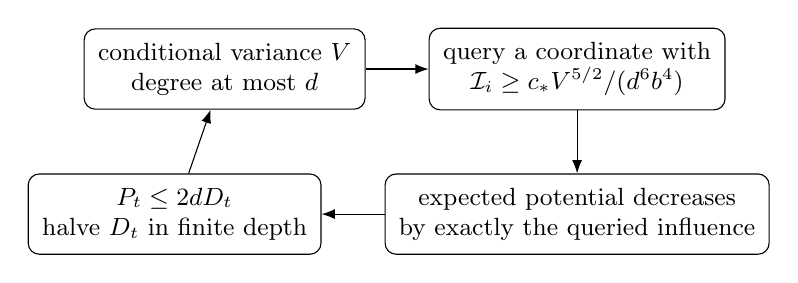
\begin{tikzpicture}[>=Latex,box/.style={draw,rounded corners,align=center,inner sep=5pt,font=\small}]
\node[box] (v) {conditional variance $V$\\degree at most $d$};
\node[box,right=8mm of v] (i) {query a coordinate with\\$\cI_i\ge c_*V^{5/2}/(d^6b^4)$};
\node[box,below=8mm of i] (p) {expected potential decreases\\by exactly the queried influence};
\node[box,left=8mm of p] (d) {$P_t\le2dD_t$\\halve $D_t$ in finite depth};
\draw[->] (v)--(i);
\draw[->] (i)--(p);
\draw[->] (p)--(d);
\draw[->] (d)--(v);
\end{tikzpicture}
\caption{The potential is the sum of remaining resampling influences.
The identity for its mean decrement supplies a bound on tree depth.}
\end{figure}

\section{Normalization and dependency checks}

For $X_i\sim\operatorname{Bernoulli}(p_i)$ and
$\Delta_i f=f(x_{-i},1)-f(x_{-i},0)$, direct conditioning gives
\[
 \cI_i(f)=2p_i(1-p_i)\E_{X_{-i}}(\Delta_i f)^2,
 \qquad\cL_i(f)=2p_i(1-p_i)\E_{X_{-i}}|\Delta_i f|.
\]
These formulas remain valid at $p_i=0,1$. At $p_i=1/2$ the factor is
$1/2$. In the $\{-1,1\}$ convention using
$\E((f(x)-f(x^{\oplus i}))/2)^2$, the resampling influence is twice
that convention's influence.

Appendix~\ref{app:determinant} gives the full determinant derivation of
Proposition~\ref{prop:external}.
Appendix~\ref{app:analytic} proves the previously published row bound
of Proposition~\ref{prop:rows}.
All uses of product independence, including conditional orientations,
the variance identity and the query potential, are written out above.
The supplementary Python file checks the exact rational identities and
finite instances; these checks supplement the proofs.

The theorem proved here is the finite-product influence statement with
variance exponent $5/2$, and its proof uses no unproved conjecture.

\section*{Declarations}

\subsection*{Data availability} No data sets were used. The Python program that checks the exact identities and finite instances, together with its output, is included with this preprint as supplementary material and archived with the source of this paper at doi:10.5281/zenodo.24124921.

\subsection*{Funding} No funding was received for this work.

\subsection*{Competing interests} The author declares no competing interests.

\subsection*{Use of artificial intelligence} AI coding assistants were used to write and test the checking program and to check the bibliography. All mathematical arguments were written and verified by the author, who takes full responsibility for the content.

\begin{thebibliography}{9}
\bibitem{AA}
S. Aaronson and A. Ambainis,
\emph{The need for structure in quantum speedups},
Theory of Computing \textbf{10} (2014), 133--166.
\href{https://doi.org/10.4086/toc.2014.v010a006}{doi:10.4086/toc.2014.v010a006}.

\bibitem{ABD}
A. Agarwal and S. Ben-David,
\emph{Oracle separations for the quantum-classical polynomial hierarchy},
17th Innovations in Theoretical Computer Science Conference,
LIPIcs \textbf{362} (2026), article 2.
\href{https://doi.org/10.4230/LIPIcs.ITCS.2026.2}{doi:10.4230/LIPIcs.ITCS.2026.2}.
The full version is \href{https://arxiv.org/abs/2410.19062v2}{arXiv:2410.19062v2}.

\bibitem{BBCMW}
R. Beals, H. Buhrman, R. Cleve, M. Mosca and R. de Wolf,
\emph{Quantum lower bounds by polynomials},
Journal of the ACM \textbf{48} (2001), 778--797.
\href{https://doi.org/10.1145/502090.502097}{doi:10.1145/502090.502097}.
\href{https://arxiv.org/abs/quant-ph/9802049}{arXiv:quant-ph/9802049}.

\bibitem{FHKL}
Y. Filmus, H. Hatami, N. Keller and N. Lifshitz,
\emph{On the sum of the $L_1$ influences of bounded functions},
Israel Journal of Mathematics \textbf{214} (2016), 167--192.
\href{https://doi.org/10.1007/s11856-016-1355-0}{doi:10.1007/s11856-016-1355-0}.

\bibitem{GMNR}
U. Girish, K. Mittal, B. Nehoran and R. Raz,
\emph{Distributional variants of the Aaronson--Ambainis conjecture},
preprint, 2026.
\href{https://arxiv.org/abs/2609.35327v1}{arXiv:2609.35327v1}.

\bibitem{Turturean}
D. Turturean,
\emph{A proof of the Aaronson--Ambainis conjecture},
preprint and accompanying formalization, November 2026.
\url{https://github.com/physical-superintelligence/aaronson-ambainis}.
\end{thebibliography}
\end{document}
